% !TEX TS-program = pdflatex
\documentclass[11pt]{article}

% -------------------- Packages --------------------
\usepackage[a4paper,margin=1in]{geometry}
\usepackage{amsmath,amssymb}
\usepackage[T1]{fontenc}
\usepackage{lmodern}
\usepackage{xcolor}
\usepackage{tcolorbox}
\tcbuselibrary{skins,breakable}
\usepackage{enumitem}
\usepackage{hyperref}
\usepackage{tikz}
\usetikzlibrary{calc,angles,quotes,intersections}
\usepackage{multicol}

\pagestyle{empty}

% -------------------- Dark Theme Colors --------------------
\definecolor{bg}{HTML}{000000}
\definecolor{pairbg}{HTML}{121212}
\definecolor{solbg}{HTML}{0A0A0A}
\definecolor{border}{HTML}{2A2A2A}
\definecolor{text}{HTML}{FFFFFF}
\definecolor{muted}{HTML}{C9CDD3}
\definecolor{gold}{HTML}{FFD700}
\definecolor{green}{HTML}{4ADE80}
\definecolor{cyan}{HTML}{38BDF8}

\pagecolor{bg}
\color{text}

\hypersetup{
  colorlinks=true,
  linkcolor=cyan,
  urlcolor=cyan
}

\setlength{\parindent}{0pt}
\setlength{\parskip}{10pt}

\setlist[itemize]{left=1.4em,itemsep=6pt,topsep=6pt}
\setlist[enumerate]{left=1.6em,itemsep=4pt,topsep=4pt}

% -------------------- tcolorbox Base --------------------
\tcbset{
  enhanced,
  breakable,
  arc=12pt,
  boxrule=0.8pt,
  left=16pt,right=16pt,top=12pt,bottom=12pt
}

\newtcolorbox{QAPair}[1]{%
  colback=pairbg,
  colbacklower=solbg,
  colframe=border,
  coltext=text,
  title=\textcolor{gold}{\bfseries #1},
  fonttitle=\bfseries,
  coltitle=text,
  segmentation style={draw=border, dashed, line width=0.6pt},
}

% Visible text inside this box (fix)
\newtcolorbox{QuickBox}{%
  colback=pairbg,
  colframe=cyan,
  coltext=text,
  fontupper=\color{text},
  borderline north={4pt}{0pt}{cyan},
  arc=14pt,
  boxrule=0.8pt
}

% Helper for step headings
\newcommand{\Step}[1]{\textcolor{muted}{\textbf{Step #1:}}}

% -------------------- TikZ styles --------------------
\tikzset{
  triEdge/.style={draw=text, line width=0.95pt, line cap=round, line join=round},
  helper/.style={draw=muted, dashed, line width=0.65pt},
  callout/.style={draw=border, rounded corners=8pt, fill=solbg, inner sep=6pt, align=left},
  goldLbl/.style={text=gold, font=\small\bfseries},
  cyanLbl/.style={text=cyan, font=\small\bfseries},
  mutedLbl/.style={text=muted, font=\small},
  dot/.style={circle, fill=cyan, inner sep=1.2pt},
}

% ============================================================
% Shared triangle coordinates + centers (illustrative)
% ============================================================
\newcommand{\TriCoordsABC}{%
  \coordinate (A) at (0,0);
  \coordinate (B) at (5,0);
  \coordinate (C) at (1.5,3);
}
\newcommand{\TriCentersIO}{%
  \coordinate (I) at (1.872,1.157); % incenter-ish
  \coordinate (O) at (2.5,0.625);   % circumcenter-ish
}

% -------------------- Concept boxes for Quick formulas --------------------
\newtcolorbox{ConceptBox}[1]{%
  colback=solbg,
  colframe=border,
  coltext=text,
  arc=14pt,
  boxrule=0.8pt,
  left=14pt,right=14pt,top=10pt,bottom=10pt,
  breakable,
  title=\textcolor{gold}{\bfseries #1},
  fonttitle=\bfseries,
  coltitle=text,
}

% ============================================================
% Quick-formula diagrams (each concept separate, centered)
% ============================================================
\newcommand{\QDiagSides}{%
\begin{tikzpicture}[scale=0.95]
  \TriCoordsABC
  \draw[triEdge] (A)--(B)--(C)--cycle;

  \node[cyanLbl, below left]  at (A) {$A$};
  \node[cyanLbl, below right] at (B) {$B$};
  \node[cyanLbl, above]       at (C) {$C$};

  \node[goldLbl] at ($(B)!0.52!(C)+(0.55,0.10)$) {$a$};
  \node[goldLbl] at ($(C)!0.52!(A)+(-0.65,0.10)$) {$b$};
  \node[goldLbl] at ($(A)!0.52!(B)+(0,-0.35)$) {$c$};
\end{tikzpicture}%
}

\newcommand{\QDiagHeron}{%
\begin{tikzpicture}[scale=0.95]
  \TriCoordsABC
  \draw[triEdge] (A)--(B)--(C)--cycle;

  \node[cyanLbl, below left]  at (A) {$A$};
  \node[cyanLbl, below right] at (B) {$B$};
  \node[cyanLbl, above]       at (C) {$C$};

  \node[goldLbl] at (2.15,1.35) {$\Delta$};
  \node[mutedLbl] at (2.15,1.05) {Area};
\end{tikzpicture}%
}

\newcommand{\QDiagInradius}{%
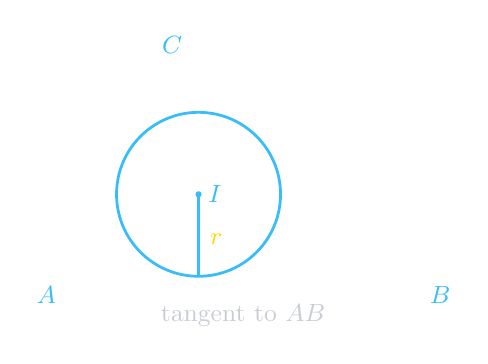
\begin{tikzpicture}[scale=0.90]
  \TriCoordsABC
  \TriCentersIO
  \draw[triEdge] (A)--(B)--(C)--cycle;

  \node[cyanLbl, below left]  at (A) {$A$};
  \node[cyanLbl, below right] at (B) {$B$};
  \node[cyanLbl, above]       at (C) {$C$};

  \draw[draw=cyan, line width=1.0pt] (I) circle (1.157);
  \fill[cyan] (I) circle (1.25pt);
  \node[cyanLbl, right] at (I) {$I$};

  \draw[draw=cyan, line width=0.95pt] (I)--(I |- A);
  \node[goldLbl] at ($(I)!0.55!(I |- A)+(0.25,0)$) {$r$};

  \node[mutedLbl] at ($(A)!0.5!(B)+(0,-0.55)$) {tangent to $AB$};
\end{tikzpicture}%
}

\newcommand{\QDiagCircumradius}{%
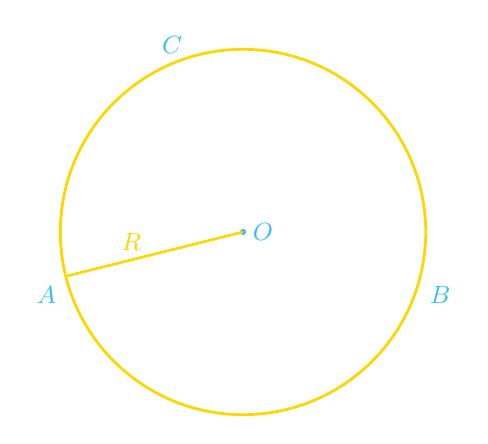
\begin{tikzpicture}[scale=0.90]
  \TriCoordsABC
  \TriCentersIO
  \draw[triEdge] (A)--(B)--(C)--cycle;

  \node[cyanLbl, below left]  at (A) {$A$};
  \node[cyanLbl, below right] at (B) {$B$};
  \node[cyanLbl, above]       at (C) {$C$};

  \draw[draw=gold, line width=1.0pt] (O) circle (2.578);
  \fill[cyan] (O) circle (1.25pt);
  \node[cyanLbl, right] at (O) {$O$};

  \draw[draw=gold, line width=0.95pt] (O)--(A);
  \node[goldLbl] at ($(O)!0.55!(A)+(-0.2,0.2)$) {$R$};
\end{tikzpicture}%
}

\newcommand{\QDiagSineRule}{%
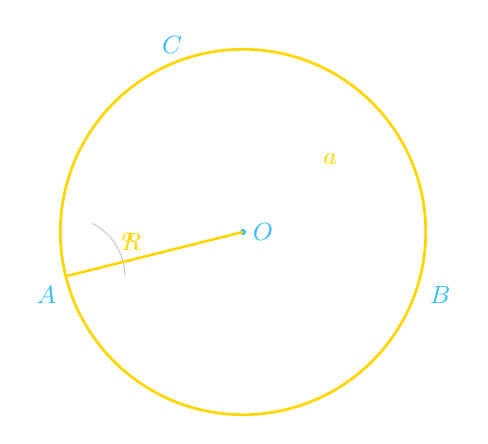
\begin{tikzpicture}[scale=0.90]
  \TriCoordsABC
  \TriCentersIO
  \draw[triEdge] (A)--(B)--(C)--cycle;

  \node[cyanLbl, below left]  at (A) {$A$};
  \node[cyanLbl, below right] at (B) {$B$};
  \node[cyanLbl, above]       at (C) {$C$};

  \draw[draw=gold, line width=1.0pt] (O) circle (2.578);
  \fill[cyan] (O) circle (1.25pt);
  \node[cyanLbl, right] at (O) {$O$};

  \node[goldLbl] at ($(B)!0.52!(C)+(0.55,0.10)$) {$a$};

  \pic[draw=muted, angle radius=7.5mm, angle eccentricity=1.25,
       "{\scriptsize\textcolor{gold}{$\alpha$}}"] {angle = B--A--C};

  \draw[draw=gold, line width=0.95pt] (O)--(A);
  \node[goldLbl] at ($(O)!0.55!(A)+(-0.2,0.2)$) {$R$};
\end{tikzpicture}%
}

\newcommand{\QDiagExradius}{%
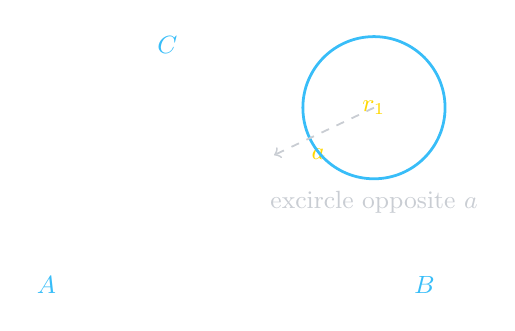
\begin{tikzpicture}[scale=0.86]
  \TriCoordsABC
  \draw[triEdge] (A)--(B)--(C)--cycle;

  \node[cyanLbl, below left]  at (A) {$A$};
  \node[cyanLbl, below right] at (B) {$B$};
  \node[cyanLbl, above]       at (C) {$C$};

  \node[goldLbl] at ($(B)!0.52!(C)+(0.55,0.10)$) {$a$};

  \coordinate (Ia) at (4.55,2.35);
  \draw[draw=cyan, line width=1.0pt] (Ia) circle (1.05);
  \node[goldLbl] at (Ia) {$r_1$};

  \draw[helper,->] (Ia) -- ($(B)!0.55!(C)$);
  \node[mutedLbl] at (4.55,0.95) {excircle opposite $a$};
\end{tikzpicture}%
}

\newcommand{\QDiagHalfAngle}{%
\begin{tikzpicture}[scale=0.95]
  \TriCoordsABC
  \draw[triEdge] (A)--(B)--(C)--cycle;

  \node[cyanLbl, below left]  at (A) {$A$};
  \node[cyanLbl, below right] at (B) {$B$};
  \node[cyanLbl, above]       at (C) {$C$};

  \coordinate (D) at ($(B)!0.50!(C)$);
  \draw[helper] (A)--(D);

  \node[goldLbl] at ($(A)+(0.70,0.60)$) {$\alpha/2$};

  \pic[draw=muted, angle radius=7.5mm, angle eccentricity=1.25,
       "{\scriptsize\textcolor{gold}{$\alpha$}}"] {angle = B--A--C};
\end{tikzpicture}%
}

% ============================================================
% (Optional) Per-question diagram macros used in solutions
% ============================================================
\newcommand{\DiagNumericAllRadii}[3]{%
\begin{tikzpicture}[scale=0.88, every node/.style={text=text}]
  \TriCoordsABC
  \TriCentersIO

  \draw[triEdge] (A)--(B)--(C)--cycle;

  \node[cyanLbl, below left]  at (A) {$A$};
  \node[cyanLbl, below right] at (B) {$B$};
  \node[cyanLbl, above]       at (C) {$C$};

  % Numeric side labels
  \node[goldLbl] at ($(B)!0.52!(C)+(0.70,0.12)$) {$a=#1$};
  \node[goldLbl] at ($(C)!0.52!(A)+(-0.90,0.12)$) {$b=#2$};
  \node[goldLbl] at ($(A)!0.52!(B)+(0,-0.45)$) {$c=#3$};

  % Incircle + circumcircle (illustrative)
  \draw[draw=cyan, line width=0.95pt] (I) circle (1.157);
  \draw[draw=gold, line width=0.95pt] (O) circle (2.578);

  % Centers
  \fill[cyan] (I) circle (1.2pt);
  \fill[cyan] (O) circle (1.2pt);
  \node[cyanLbl, right] at (I) {$I$};
  \node[cyanLbl, right] at (O) {$O$};

  % Radii indicators
  \draw[draw=cyan, line width=0.9pt] (I)--(I |- A);
  \node[goldLbl] at ($(I)!0.55!(I |- A)+(0.25,0)$) {$r$};

  \draw[draw=gold, line width=0.9pt] (O)--(A);
  \node[goldLbl] at ($(O)!0.55!(A)+(-0.2,0.2)$) {$R$};

  % Exradii labels (conceptual)
  \draw[helper, ->] ($(B)!0.52!(C)+(1.55,0.35)$) -- ($(B)!0.52!(C)+(0.2,0.05)$);
  \node[goldLbl, anchor=west] at ($(B)!0.52!(C)+(1.55,0.35)$) {$r_1$ (opp.\ $a$)};

  \draw[helper, ->] ($(C)!0.52!(A)+(-1.75,0.35)$) -- ($(C)!0.52!(A)+(-0.25,0.05)$);
  \node[goldLbl, anchor=east] at ($(C)!0.52!(A)+(-1.75,0.35)$) {$r_2$ (opp.\ $b$)};

  \draw[helper, ->] ($(A)!0.52!(B)+(0,-1.20)$) -- ($(A)!0.52!(B)+(0,-0.20)$);
  \node[goldLbl, anchor=north] at ($(A)!0.52!(B)+(0,-1.20)$) {$r_3$ (opp.\ $c$)};

\end{tikzpicture}%
}

\newcommand{\DiagInCircum}{%
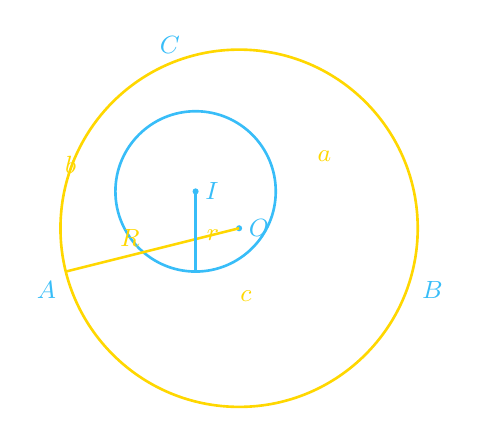
\begin{tikzpicture}[scale=0.88, every node/.style={text=text}]
  \TriCoordsABC
  \TriCentersIO

  \draw[triEdge] (A)--(B)--(C)--cycle;

  \node[cyanLbl, below left]  at (A) {$A$};
  \node[cyanLbl, below right] at (B) {$B$};
  \node[cyanLbl, above]       at (C) {$C$};

  % Side labels
  \node[goldLbl] at ($(B)!0.52!(C)+(0.55,0.10)$) {$a$};
  \node[goldLbl] at ($(C)!0.52!(A)+(-0.65,0.10)$) {$b$};
  \node[goldLbl] at ($(A)!0.52!(B)+(0,-0.35)$) {$c$};

  % Incircle
  \draw[draw=cyan, line width=0.95pt] (I) circle (1.157);
  \fill[cyan] (I) circle (1.25pt);
  \node[cyanLbl, right] at (I) {$I$};

  % Circumcircle
  \draw[draw=gold, line width=0.95pt] (O) circle (2.578);
  \fill[cyan] (O) circle (1.25pt);
  \node[cyanLbl, right] at (O) {$O$};

  \draw[draw=gold, line width=0.9pt] (O)--(A);
  \node[goldLbl] at ($(O)!0.55!(A)+(-0.2,0.2)$) {$R$};

  \draw[draw=cyan, line width=0.9pt] (I)--(I |- A);
  \node[goldLbl] at ($(I)!0.55!(I |- A)+(0.25,0)$) {$r$};
\end{tikzpicture}%
}

\newcommand{\DiagHalfAngles}{%
\begin{tikzpicture}[scale=0.90, every node/.style={text=text}]
  \TriCoordsABC
  \draw[triEdge] (A)--(B)--(C)--cycle;

  \node[cyanLbl, below left]  at (A) {$A$};
  \node[cyanLbl, below right] at (B) {$B$};
  \node[cyanLbl, above]       at (C) {$C$};

  \coordinate (D) at ($(B)!0.50!(C)$);
  \coordinate (E) at ($(C)!0.50!(A)$);
  \coordinate (F) at ($(A)!0.50!(B)$);

  \draw[helper] (A)--(D);
  \draw[helper] (B)--(E);
  \draw[helper] (C)--(F);

  \node[goldLbl] at ($(A)+(0.55,0.55)$) {$\dfrac{\alpha}{2}$};
  \node[goldLbl] at ($(B)+(-0.60,0.55)$) {$\dfrac{\beta}{2}$};
  \node[goldLbl] at ($(C)+(0.05,-0.70)$) {$\dfrac{\gamma}{2}$};

  \pic[draw=muted, angle radius=7.5mm, angle eccentricity=1.28,
       "{\scriptsize\textcolor{gold}{$\alpha$}}"] {angle = B--A--C};
  \pic[draw=muted, angle radius=7.5mm, angle eccentricity=1.28,
       "{\scriptsize\textcolor{gold}{$\beta$}}"]  {angle = C--B--A};
  \pic[draw=muted, angle radius=7.5mm, angle eccentricity=1.28,
       "{\scriptsize\textcolor{gold}{$\gamma$}}"] {angle = A--C--B};
\end{tikzpicture}%
}

% ============================================================
\begin{document}

\begin{center}
{\LARGE\bfseries \textcolor{gold}{Exercise 8.5 --- Solutions}}\\[-2pt]
\end{center}

% ============================================================
% CLEAN QUICK FORMULAS (NO OVERFLOW, ONE CONCEPT PER LINE)
\begin{QuickBox}
{\color{cyan}\bfseries Quick formulas (clean + readable)}\par\medskip

\begin{ConceptBox}{1) Semi-perimeter $S$}
\[
S=\frac{a+b+c}{2}
\]
\begin{center}
\QDiagSides
\end{center}
\end{ConceptBox}

\begin{ConceptBox}{2) Heron's formula (Area)}
\[
\Delta=\sqrt{S(S-a)(S-b)(S-c)}
\]
\begin{center}
\QDiagHeron
\end{center}
\end{ConceptBox}

\begin{ConceptBox}{3) Inradius $r$}
\[
\Delta=rS
\qquad\Rightarrow\qquad
r=\frac{\Delta}{S}
\]
\begin{center}
\QDiagInradius
\end{center}
\end{ConceptBox}

\begin{ConceptBox}{4) Circumradius $R$}
\[
\Delta=\frac{abc}{4R}
\qquad\Rightarrow\qquad
R=\frac{abc}{4\Delta}
\]
\begin{center}
\QDiagCircumradius
\end{center}
\end{ConceptBox}

\begin{ConceptBox}{5) Sine rule (uses $R$)}
\[
\begin{aligned}
a&=2R\sin\alpha,\\
b&=2R\sin\beta,\\
c&=2R\sin\gamma.
\end{aligned}
\]
\begin{center}
\QDiagSineRule
\end{center}
\end{ConceptBox}

\begin{ConceptBox}{6) Exradii $r_1,r_2,r_3$}
\[
\begin{aligned}
r_1&=\frac{\Delta}{S-a},\\
r_2&=\frac{\Delta}{S-b},\\
r_3&=\frac{\Delta}{S-c}.
\end{aligned}
\]
\begin{center}
\QDiagExradius
\end{center}
{\small\textcolor{muted}{(Similarly, the excircle opposite $b$ gives $r_2$, and opposite $c$ gives $r_3$.)}}
\end{ConceptBox}

\begin{ConceptBox}{7) Half-angle formulas (no overflow)}
\[
\begin{aligned}
\sin\frac{\alpha}{2}&=\sqrt{\frac{(S-b)(S-c)}{bc}},\\
\cos\frac{\alpha}{2}&=\sqrt{\frac{S(S-a)}{bc}},\\
\tan\frac{\alpha}{2}&=\frac{r}{S-a}.
\end{aligned}
\]
{\small\textcolor{muted}{(Cyclic for $\beta$ and $\gamma$.)}}
\begin{center}
\QDiagHalfAngle
\end{center}
\end{ConceptBox}

\end{QuickBox}

% ============================================================
% Q1
\begin{QAPair}{Question 1 (i)}
\textcolor{gold}{\bfseries Question:} Find $r,\;R,\;r_1,\;r_2,\;r_3$ when $a=10,\;b=13,\;c=17$.\\
\tcblower
\textcolor{green}{\bfseries Diagram (map of radii):}\par
\begin{center}
\DiagNumericAllRadii{10}{13}{17}
\end{center}

\textcolor{green}{\bfseries Answer:}
Let $S=\dfrac{a+b+c}{2}$ and $\Delta=\sqrt{S(S-a)(S-b)(S-c)}$.
\[
\begin{aligned}
\Step{1}\;& S=\frac{10+13+17}{2}=20.\\
\Step{2}\;& \Delta=\sqrt{20\cdot 10\cdot 7\cdot 3}=\sqrt{4200}=10\sqrt{42}.\\
\Step{3}\;& r=\frac{\Delta}{S}=\frac{10\sqrt{42}}{20}=\frac{\sqrt{42}}{2}\approx 3.240.\\
\Step{4}\;& R=\frac{abc}{4\Delta}=\frac{10\cdot 13\cdot 17}{4(10\sqrt{42})}
=\frac{221}{4\sqrt{42}}=\frac{221\sqrt{42}}{168}\approx 8.525.\\
\Step{5}\;& r_1=\frac{\Delta}{S-a}=\frac{10\sqrt{42}}{10}=\sqrt{42}\approx 6.481,\\
& r_2=\frac{\Delta}{S-b}=\frac{10\sqrt{42}}{7}\approx 9.258,\\
& r_3=\frac{\Delta}{S-c}=\frac{10\sqrt{42}}{3}\approx 21.603.
\end{aligned}
\]
\end{QAPair}

\begin{QAPair}{Question 1 (ii)}
\textcolor{gold}{\bfseries Question:} Find $r,\;R,\;r_1,\;r_2,\;r_3$ when $a=22,\;b=24,\;c=30$.\\
\tcblower
\textcolor{green}{\bfseries Diagram (map of radii):}\par
\begin{center}
\DiagNumericAllRadii{22}{24}{30}
\end{center}

\textcolor{green}{\bfseries Answer:}
\[
\begin{aligned}
\Step{1}\;& S=\frac{22+24+30}{2}=38.\\
\Step{2}\;& \Delta=\sqrt{38\cdot 16\cdot 14\cdot 8}
=\sqrt{68096}=16\sqrt{266}.\\
\Step{3}\;& r=\frac{\Delta}{S}=\frac{16\sqrt{266}}{38}=\frac{8\sqrt{266}}{19}\approx 6.867.\\
\Step{4}\;& R=\frac{abc}{4\Delta}=\frac{22\cdot 24\cdot 30}{4(16\sqrt{266})}
=\frac{247.5}{\sqrt{266}}=\frac{495}{2\sqrt{266}}\approx 15.175.\\
\Step{5}\;& r_1=\frac{\Delta}{S-a}=\frac{16\sqrt{266}}{16}=\sqrt{266}\approx 16.310,\\
& r_2=\frac{\Delta}{S-b}=\frac{16\sqrt{266}}{14}=\frac{8\sqrt{266}}{7}\approx 18.639,\\
& r_3=\frac{\Delta}{S-c}=\frac{16\sqrt{266}}{8}=2\sqrt{266}\approx 32.619.
\end{aligned}
\]
\end{QAPair}

\begin{QAPair}{Question 1 (iii)}
\textcolor{gold}{\bfseries Question:} Find $r,\;R,\;r_1,\;r_2,\;r_3$ when $a=3,\;b=4,\;c=5$.\\
\tcblower
\textcolor{green}{\bfseries Diagram (map of radii):}\par
\begin{center}
\DiagNumericAllRadii{3}{4}{5}
\end{center}

\textcolor{green}{\bfseries Answer:}
\[
\begin{aligned}
\Step{1}\;& S=\frac{3+4+5}{2}=6.\\
\Step{2}\;& \Delta=\sqrt{6\cdot 3\cdot 2\cdot 1}=6.\\
\Step{3}\;& r=\frac{\Delta}{S}=1.\\
\Step{4}\;& R=\frac{abc}{4\Delta}=\frac{3\cdot 4\cdot 5}{24}=\frac52=2.5.\\
\Step{5}\;& r_1=\frac{\Delta}{S-a}=2,\quad
r_2=\frac{\Delta}{S-b}=3,\quad
r_3=\frac{\Delta}{S-c}=6.
\end{aligned}
\]
\end{QAPair}

\begin{QAPair}{Question 1 (iv)}
\textcolor{gold}{\bfseries Question:} Find $r,\;R,\;r_1,\;r_2,\;r_3$ when $a=50,\;b=60,\;c=70$.\\
\tcblower
\textcolor{green}{\bfseries Diagram (map of radii):}\par
\begin{center}
\DiagNumericAllRadii{50}{60}{70}
\end{center}

\textcolor{green}{\bfseries Answer:}
\[
\begin{aligned}
\Step{1}\;& S=\frac{50+60+70}{2}=90.\\
\Step{2}\;& \Delta=\sqrt{90\cdot 40\cdot 30\cdot 20}
=\sqrt{2160000}=600\sqrt6.\\
\Step{3}\;& r=\frac{\Delta}{S}=\frac{600\sqrt6}{90}=\frac{20\sqrt6}{3}\approx 16.330.\\
\Step{4}\;& R=\frac{abc}{4\Delta}=\frac{50\cdot60\cdot70}{4(600\sqrt6)}
=\frac{175}{2\sqrt6}=\frac{175\sqrt6}{12}\approx 35.722.\\
\Step{5}\;& r_1=\frac{\Delta}{S-a}=\frac{600\sqrt6}{40}=15\sqrt6\approx 36.742,\\
& r_2=\frac{600\sqrt6}{30}=20\sqrt6\approx 48.990,\\
& r_3=\frac{600\sqrt6}{20}=30\sqrt6\approx 73.485.
\end{aligned}
\]
\end{QAPair}

% ============================================================
% Q2
\begin{QAPair}{Question 2 (i)}
\textcolor{gold}{\bfseries Question:} If $ABC$ is an equilateral triangle, prove that $r:R:r_1=1:2:3$.\\
\tcblower
\textcolor{green}{\bfseries Diagram:}\par
\begin{center}
\DiagInCircum
\end{center}

\textcolor{green}{\bfseries Answer:}
Let each side be $a$. Then
\[
S=\frac{3a}{2},\qquad \Delta=\frac{\sqrt3}{4}a^2.
\]
\[
\begin{aligned}
\Step{1}\;& r=\frac{\Delta}{S}
=\frac{\frac{\sqrt3}{4}a^2}{\frac{3a}{2}}
=\frac{\sqrt3}{6}a.\\
\Step{2}\;& R=\frac{a^3}{4\Delta}=\frac{a^3}{4\cdot\frac{\sqrt3}{4}a^2}
=\frac{a}{\sqrt3}=2r.\\
\Step{3}\;& r_1=\frac{\Delta}{S-a}
=\frac{\frac{\sqrt3}{4}a^2}{\frac{a}{2}}
=\frac{\sqrt3}{2}a=3r.
\end{aligned}
\]
Hence $r:R:r_1=1:2:3$.
\end{QAPair}

\begin{QAPair}{Question 2 (ii)}
\textcolor{gold}{\bfseries Question:} If $ABC$ is an equilateral triangle, prove that $r_1:r_2:r_3=1:1:1$.\\
\tcblower
\textcolor{green}{\bfseries Diagram:}\par
\begin{center}
\DiagInCircum
\end{center}

\textcolor{green}{\bfseries Answer:}
In an equilateral triangle $a=b=c$, so
\[
S-a=S-b=S-c=\frac{a}{2}.
\]
Therefore,
\[
r_1=\frac{\Delta}{S-a}=\frac{\Delta}{S-b}=\frac{\Delta}{S-c}=r_2=r_3
\quad\Rightarrow\quad r_1:r_2:r_3=1:1:1.
\]
\end{QAPair}

% ============================================================
% Q3
\begin{QAPair}{Question 3 (i)}
\textcolor{gold}{\bfseries Question:} Show that
\[
\frac1{ab}+\frac1{bc}+\frac1{ca}
=\frac{2S}{abc}
=\frac{1}{2rR}.
\]
\tcblower
\textcolor{green}{\bfseries Diagram:}\par
\begin{center}
\DiagInCircum
\end{center}

\textcolor{green}{\bfseries Answer:}
\[
\begin{aligned}
\Step{1}\;& \frac1{ab}+\frac1{bc}+\frac1{ca}
=\frac{a+b+c}{abc}
=\frac{2S}{abc}.\\
\Step{2}\;& abc=4R\Delta,\ \Delta=rS.\\
\Step{3}\;& \frac{2S}{abc}=\frac{2S}{4R\Delta}
=\frac{S}{2R\Delta}
=\frac{S}{2R(rS)}=\frac{1}{2rR}.
\end{aligned}
\]
\end{QAPair}

\begin{QAPair}{Question 3 (ii)}
\textcolor{gold}{\bfseries Question:} Show that
\[
\frac1{r_1}+\frac1{r_2}+\frac1{r_3}=\frac{S}{\Delta}.
\]
\tcblower
\textcolor{green}{\bfseries Diagram:}\par
\begin{center}
\QDiagExradius
\end{center}

\textcolor{green}{\bfseries Answer:}
Since $r_1=\dfrac{\Delta}{S-a}$ etc.,
\[
\begin{aligned}
\Step{1}\;& \frac1{r_1}+\frac1{r_2}+\frac1{r_3}
=\frac{S-a}{\Delta}+\frac{S-b}{\Delta}+\frac{S-c}{\Delta}\\
\Step{2}\;&=\frac{3S-(a+b+c)}{\Delta}
=\frac{3S-2S}{\Delta}
=\frac{S}{\Delta}.
\end{aligned}
\]
\end{QAPair}

\begin{QAPair}{Question 3 (iii)}
\textcolor{gold}{\bfseries Question:} Show that $r_1r_2+r_2r_3+r_3r_1=S^2$.\\
\tcblower
\textcolor{green}{\bfseries Diagram:}\par
\begin{center}
\QDiagExradius
\end{center}

\textcolor{green}{\bfseries Answer:}
Let $x=S-a,\;y=S-b,\;z=S-c$. Then $\Delta^2=Sxyz$ (Heron).
Also $r_1=\dfrac{\Delta}{x}$, $r_2=\dfrac{\Delta}{y}$, $r_3=\dfrac{\Delta}{z}$.
\[
\begin{aligned}
\Step{1}\;& r_1r_2+r_2r_3+r_3r_1
=\Delta^2\!\left(\frac1{xy}+\frac1{yz}+\frac1{zx}\right)\\
\Step{2}\;&=\Delta^2\cdot \frac{x+y+z}{xyz}
=\Delta^2\cdot \frac{S}{xyz}
=\bigl(Sxyz\bigr)\cdot \frac{S}{xyz}
=S^2.
\end{aligned}
\]
\end{QAPair}

\begin{QAPair}{Question 3 (iv)}
\textcolor{gold}{\bfseries Question:} Show that $r_1+r_2+r_3-r=4R$.\\
\tcblower
\textcolor{green}{\bfseries Diagram:}\par
\begin{center}
\DiagInCircum
\end{center}

\textcolor{green}{\bfseries Answer:}
Let $x=S-a,\;y=S-b,\;z=S-c$ so that $\Delta^2=Sxyz$ and $r=\Delta/S$.
\[
\begin{aligned}
\Step{1}\;& r_1+r_2+r_3-r
=\Delta\!\left(\frac1x+\frac1y+\frac1z-\frac1S\right)\\
\Step{2}\;&=\Delta\!\left(\frac{xy+yz+zx}{xyz}-\frac1S\right)
=\Delta\!\left(\frac{S(xy+yz+zx)-xyz}{Sxyz}\right).
\end{aligned}
\]
But $\;S(xy+yz+zx)-xyz=abc\;$, so
\[
r_1+r_2+r_3-r
=\Delta\cdot \frac{abc}{Sxyz}
=\Delta\cdot \frac{abc}{\Delta^2}
=\frac{abc}{\Delta}
=4R.
\]
\end{QAPair}

\begin{QAPair}{Question 3 (v)}
\textcolor{gold}{\bfseries Question:} Show that $\sqrt{rr_1r_2r_3}=\Delta$.\\
\tcblower
\textcolor{green}{\bfseries Diagram:}\par
\begin{center}
\DiagInCircum
\end{center}

\textcolor{green}{\bfseries Answer:}
Using $r=\dfrac{\Delta}{S}$ and $r_1r_2r_3=\dfrac{\Delta^3}{(S-a)(S-b)(S-c)}$:
\[
\begin{aligned}
\Step{1}\;& rr_1r_2r_3
=\frac{\Delta}{S}\cdot \frac{\Delta^3}{(S-a)(S-b)(S-c)}
=\frac{\Delta^4}{S(S-a)(S-b)(S-c)}.\\
\Step{2}\;& \Delta^2=S(S-a)(S-b)(S-c).\\
\Step{3}\;& \Rightarrow\; rr_1r_2r_3=\Delta^2
\quad\Rightarrow\quad \sqrt{rr_1r_2r_3}=\Delta.
\end{aligned}
\]
\end{QAPair}

\begin{QAPair}{Question 3 (vi)}
\textcolor{gold}{\bfseries Question:} Show that $r_1r_2r_3=rS^2$.\\
\tcblower
\textcolor{green}{\bfseries Diagram:}\par
\begin{center}
\QDiagExradius
\end{center}

\textcolor{green}{\bfseries Answer:}
\[
\begin{aligned}
\Step{1}\;& r_1r_2r_3=\frac{\Delta}{S-a}\cdot\frac{\Delta}{S-b}\cdot\frac{\Delta}{S-c}
=\frac{\Delta^3}{(S-a)(S-b)(S-c)}.\\
\Step{2}\;& \Delta^2=S(S-a)(S-b)(S-c)\Rightarrow (S-a)(S-b)(S-c)=\frac{\Delta^2}{S}.\\
\Step{3}\;& r_1r_2r_3=\frac{\Delta^3}{\Delta^2/S}=\Delta S=(\Delta/S)S^2=rS^2.
\end{aligned}
\]
\end{QAPair}

% ============================================================
% Q4
\begin{QAPair}{Question 4}
\textcolor{gold}{\bfseries Question:} Show that $(\sin\alpha+\sin\beta+\sin\gamma)=\dfrac{S}{R}$.\\
\tcblower
\textcolor{green}{\bfseries Diagram:}\par
\begin{center}
\QDiagSineRule
\end{center}

\textcolor{green}{\bfseries Answer:}
By the sine rule, $a=2R\sin\alpha$, $b=2R\sin\beta$, $c=2R\sin\gamma$. Hence
\[
\begin{aligned}
\Step{1}\;& \sin\alpha+\sin\beta+\sin\gamma
=\frac{a+b+c}{2R}.\\
\Step{2}\;& a+b+c=2S \Rightarrow \sin\alpha+\sin\beta+\sin\gamma=\frac{S}{R}.
\end{aligned}
\]
\end{QAPair}

% ============================================================
% Q5
\begin{QAPair}{Question 5}
\textcolor{gold}{\bfseries Question:} Prove that
\[
(r_1+r_2)\tan\frac{\gamma}{2}=(r_3-r)\cot\frac{\gamma}{2}=c.
\]
\tcblower
\textcolor{green}{\bfseries Diagram:}\par
\begin{center}
\DiagHalfAngles
\end{center}

\textcolor{green}{\bfseries Answer:}
We use $\tan\frac{\gamma}{2}=\dfrac{r}{S-c}$ and $\cot\frac{\gamma}{2}=\dfrac{S-c}{r}$.

\[
\begin{aligned}
\Step{1}\;& (r_1+r_2)\tan\frac{\gamma}{2}
=\left(\frac{\Delta}{S-a}+\frac{\Delta}{S-b}\right)\frac{r}{S-c}\\
&=\Delta r\cdot \frac{(S-b)+(S-a)}{(S-a)(S-b)(S-c)}
=\Delta r\cdot \frac{c}{(S-a)(S-b)(S-c)}.
\end{aligned}
\]
But $(S-a)(S-b)(S-c)=\dfrac{\Delta^2}{S}$, so
\[
(r_1+r_2)\tan\frac{\gamma}{2}
=\Delta r\cdot \frac{c}{\Delta^2/S}
=c\cdot \frac{rS}{\Delta}=c
\quad (\because \Delta=rS).
\]

\[
\begin{aligned}
\Step{2}\;& (r_3-r)\cot\frac{\gamma}{2}
=\left(\frac{\Delta}{S-c}-\frac{\Delta}{S}\right)\frac{S-c}{r}\\
&=\Delta\left(\frac{c}{S(S-c)}\right)\frac{S-c}{r}
=\frac{\Delta c}{Sr}
=c.
\end{aligned}
\]
Hence both expressions equal $c$.
\end{QAPair}

% ============================================================
% Q6
\begin{QAPair}{Question 6 (i)}
\textcolor{gold}{\bfseries Question:} Show that
\[
4rR\cos\frac{\alpha}{2}\cos\frac{\beta}{2}\cos\frac{\gamma}{2}
= r^2\cot\frac{\alpha}{2}\cot\frac{\beta}{2}\cot\frac{\gamma}{2}
=\Delta.
\]
\tcblower
\textcolor{green}{\bfseries Diagram:}\par
\begin{center}
\DiagHalfAngles
\end{center}

\textcolor{green}{\bfseries Answer:}
Use the half-angle formulas:
\[
\cos\frac{\alpha}{2}=\sqrt{\frac{S(S-a)}{bc}},\qquad
\sin\frac{\alpha}{2}=\sqrt{\frac{(S-b)(S-c)}{bc}}
\Rightarrow
\cot\frac{\alpha}{2}=\sqrt{\frac{S(S-a)}{(S-b)(S-c)}}.
\]

\[
\begin{aligned}
\Step{1}\;& \cos\frac{\alpha}{2}\cos\frac{\beta}{2}\cos\frac{\gamma}{2}
=\sqrt{\frac{S(S-a)}{bc}\cdot\frac{S(S-b)}{ca}\cdot\frac{S(S-c)}{ab}}\\
&=\sqrt{\frac{S^3(S-a)(S-b)(S-c)}{a^2b^2c^2}}
=\frac{S\Delta}{abc}.
\end{aligned}
\]
So,
\[
4rR\prod\cos\frac{\cdot}{2}
=4\left(\frac{\Delta}{S}\right)R\left(\frac{S\Delta}{abc}\right)
=\frac{4R\Delta^2}{abc}
=\Delta
\quad (\because abc=4R\Delta).
\]

\[
\begin{aligned}
\Step{2}\;& \cot\frac{\alpha}{2}\cot\frac{\beta}{2}\cot\frac{\gamma}{2}
=\sqrt{\frac{S^3}{(S-a)(S-b)(S-c)}}
=\frac{S^2}{\Delta}.
\end{aligned}
\]
Hence
\[
r^2\prod\cot\frac{\cdot}{2}
=\left(\frac{\Delta}{S}\right)^2\cdot\frac{S^2}{\Delta}
=\Delta.
\]
\end{QAPair}

\begin{QAPair}{Question 6 (ii)}
\textcolor{gold}{\bfseries Question:} Show that
\[
r=4R\sin\frac{\alpha}{2}\sin\frac{\beta}{2}\sin\frac{\gamma}{2}
= S\tan\frac{\alpha}{2}\tan\frac{\beta}{2}\tan\frac{\gamma}{2}.
\]
\tcblower
\textcolor{green}{\bfseries Diagram:}\par
\begin{center}
\DiagHalfAngles
\end{center}

\textcolor{green}{\bfseries Answer:}
\[
\begin{aligned}
\Step{1}\;& \sin\frac{\alpha}{2}\sin\frac{\beta}{2}\sin\frac{\gamma}{2}
=\sqrt{\frac{(S-a)^2(S-b)^2(S-c)^2}{a^2b^2c^2}}
=\frac{(S-a)(S-b)(S-c)}{abc}\\
&=\frac{\Delta^2/S}{abc}
=\frac{\Delta}{4RS}.
\end{aligned}
\]
Therefore
\[
4R\sin\frac{\alpha}{2}\sin\frac{\beta}{2}\sin\frac{\gamma}{2}
=\frac{\Delta}{S}=r.
\]
Also $\tan\frac{\alpha}{2}=\frac{r}{S-a}$ etc., so
\[
\tan\frac{\alpha}{2}\tan\frac{\beta}{2}\tan\frac{\gamma}{2}
=\frac{r^3}{(S-a)(S-b)(S-c)}
=\frac{r^3}{\Delta^2/S}
=\frac{r}{S}.
\]
Hence $S\tan\frac{\alpha}{2}\tan\frac{\beta}{2}\tan\frac{\gamma}{2}=r$.
\end{QAPair}

\begin{QAPair}{Question 6 (iii)}
\textcolor{gold}{\bfseries Question:} Show that
\[
r=a\sin\frac{\beta}{2}\sin\frac{\gamma}{2}\sec\frac{\alpha}{2}
=b\sin\frac{\alpha}{2}\sin\frac{\gamma}{2}\sec\frac{\beta}{2}
=c\sin\frac{\alpha}{2}\sin\frac{\beta}{2}\sec\frac{\gamma}{2}.
\]
\tcblower
\textcolor{green}{\bfseries Diagram:}\par
\begin{center}
\DiagHalfAngles
\end{center}

\textcolor{green}{\bfseries Answer:}
We prove the first; the others follow cyclically.

Use:
\[
\sin\frac{\beta}{2}=\sqrt{\frac{(S-c)(S-a)}{ca}},\quad
\sin\frac{\gamma}{2}=\sqrt{\frac{(S-a)(S-b)}{ab}},\quad
\sec\frac{\alpha}{2}=\sqrt{\frac{bc}{S(S-a)}}.
\]
\[
\begin{aligned}
\Step{1}\;& a\sin\frac{\beta}{2}\sin\frac{\gamma}{2}\sec\frac{\alpha}{2}\\
&=(S-a)\sqrt{\frac{(S-b)(S-c)}{bc}\cdot\frac{bc}{S(S-a)}}
=\sqrt{\frac{(S-a)(S-b)(S-c)}{S}}.
\end{aligned}
\]
But $\Delta^2=S(S-a)(S-b)(S-c)$, so
\[
\sqrt{\frac{(S-a)(S-b)(S-c)}{S}}
=\frac{\Delta}{S}=r.
\]
\end{QAPair}

% ============================================================
% Q7
\begin{QAPair}{Question 7}
\textcolor{gold}{\bfseries Question:} Prove that
\[
\text{(i)}\;\;4R\sin\frac{\alpha}{2}\cos\frac{\beta}{2}\cos\frac{\gamma}{2}=r_1,\qquad
\text{(ii)}\;\;4R\cos\frac{\alpha}{2}\sin\frac{\beta}{2}\cos\frac{\gamma}{2}=r_2.
\]
(Also cyclically, $4R\cos\frac{\alpha}{2}\cos\frac{\beta}{2}\sin\frac{\gamma}{2}=r_3$.)\\
\tcblower
\textcolor{green}{\bfseries Diagram:}\par
\begin{center}
\DiagHalfAngles
\end{center}

\textcolor{green}{\bfseries Answer:}
We prove (i). Using half-angle formulas:
\[
\sin\frac{\alpha}{2}=\sqrt{\frac{(S-b)(S-c)}{bc}},\quad
\cos\frac{\beta}{2}=\sqrt{\frac{S(S-b)}{ca}},\quad
\cos\frac{\gamma}{2}=\sqrt{\frac{S(S-c)}{ab}}.
\]
\[
\begin{aligned}
\Step{1}\;& \sin\frac{\alpha}{2}\cos\frac{\beta}{2}\cos\frac{\gamma}{2}
=\sqrt{\frac{S^2(S-b)^2(S-c)^2}{a^2b^2c^2}}
=\frac{S(S-b)(S-c)}{abc}.\\
\Step{2}\;& 4R(\cdots)=4R\cdot\frac{S(S-b)(S-c)}{abc}
=\frac{S(S-b)(S-c)}{\Delta}\quad(\because abc=4R\Delta).\\
\Step{3}\;& \Delta^2=S(S-a)(S-b)(S-c)\Rightarrow S(S-b)(S-c)=\frac{\Delta^2}{S-a}.\\
\Step{4}\;& \Rightarrow\; 4R(\cdots)=\frac{\Delta}{S-a}=r_1.
\end{aligned}
\]
The other parts are analogous.
\end{QAPair}

% ============================================================
% Q8
\begin{QAPair}{Question 8}
\textcolor{gold}{\bfseries Question:} Prove that
\[
r_1=S\tan\frac{\alpha}{2},\quad
r_2=S\tan\frac{\beta}{2},\quad
r_3=S\tan\frac{\gamma}{2}.
\]
\tcblower
\textcolor{green}{\bfseries Diagram:}\par
\begin{center}
\DiagHalfAngles
\end{center}

\textcolor{green}{\bfseries Answer:}
Using $\tan\frac{\alpha}{2}=\dfrac{r}{S-a}$ and $\Delta=rS$:
\[
S\tan\frac{\alpha}{2}=S\cdot\frac{r}{S-a}
=\frac{rS}{S-a}
=\frac{\Delta}{S-a}
=r_1.
\]
Similarly, $r_2=S\tan\frac{\beta}{2}$ and $r_3=S\tan\frac{\gamma}{2}$.
\end{QAPair}

% ============================================================
% Q9
\begin{QAPair}{Question 9}
\textcolor{gold}{\bfseries Question:} Prove that
\[
r=(S-a)\tan\frac{\alpha}{2}=(S-b)\tan\frac{\beta}{2}=(S-c)\tan\frac{\gamma}{2}.
\]
\tcblower
\textcolor{green}{\bfseries Diagram:}\par
\begin{center}
\DiagHalfAngles
\end{center}

\textcolor{green}{\bfseries Answer:}
From $\tan\frac{\alpha}{2}=\dfrac{r}{S-a}$,
\[
(S-a)\tan\frac{\alpha}{2}=r.
\]
Similarly, $\tan\frac{\beta}{2}=\dfrac{r}{S-b}$ and $\tan\frac{\gamma}{2}=\dfrac{r}{S-c}$ give the other equalities.
\end{QAPair}

% ============================================================
% Q10
\begin{QAPair}{Question 10}
\textcolor{gold}{\bfseries Question:} Find the radius of in-circle and circum-circle of a triangle having sides $7\text{ cm}, 12\text{ cm}, 15\text{ cm}$.\\
\tcblower
\textcolor{green}{\bfseries Diagram (map of radii):}\par
\begin{center}
\DiagNumericAllRadii{7}{12}{15}
\end{center}

\textcolor{green}{\bfseries Answer:}
Let $a=7,\;b=12,\;c=15$.
\[
\begin{aligned}
\Step{1}\;& S=\frac{7+12+15}{2}=17.\\
\Step{2}\;& \Delta=\sqrt{17\cdot 10\cdot 5\cdot 2}=\sqrt{1700}=10\sqrt{17}.\\
\Step{3}\;& r=\frac{\Delta}{S}=\frac{10\sqrt{17}}{17}\approx 2.425\text{ cm}.\\
\Step{4}\;& R=\frac{abc}{4\Delta}=\frac{7\cdot 12\cdot 15}{4(10\sqrt{17})}
=\frac{63}{2\sqrt{17}}=\frac{63\sqrt{17}}{34}\approx 7.640\text{ cm}.
\end{aligned}
\]
\end{QAPair}

% ============================================================
% Q11
\begin{QAPair}{Question 11}
\textcolor{gold}{\bfseries Question:} The sides of a triangle are $5\text{ cm}, 9\text{ cm}, 10\text{ cm}$. Find the circumference of the ex-circle:
\[
\text{(i) opposite to smaller side}\qquad \text{(ii) opposite to larger side.}
\]
\tcblower
\textcolor{green}{\bfseries Answer:}
Take $a=5,\;b=9,\;c=10$ (so $a$ is smallest and $c$ is largest).
\[
\begin{aligned}
\Step{1}\;& S=\frac{5+9+10}{2}=12.\\
\Step{2}\;& \Delta=\sqrt{12\cdot 7\cdot 3\cdot 2}=\sqrt{504}=6\sqrt{14}.\\
\Step{3}\;& r_1=\frac{\Delta}{S-a}=\frac{6\sqrt{14}}{7},\qquad
r_3=\frac{\Delta}{S-c}=3\sqrt{14}.
\end{aligned}
\]
Circumference of a circle is $2\pi r$.
\[
\begin{aligned}
\Step{4}\;& \text{(i) Opposite smaller side }(a=5):\;\; C_1=2\pi r_1
=\frac{12\pi\sqrt{14}}{7}\ \text{cm}.\\
\Step{5}\;& \text{(ii) Opposite larger side }(c=10):\;\; C_3=2\pi r_3
=6\pi\sqrt{14}\ \text{cm}.
\end{aligned}
\]
\end{QAPair}

% ============================================================
% Q12
\begin{QAPair}{Question 12}
\textcolor{gold}{\bfseries Question:} Find the area and circumference of the in-circle of a triangle having sides $2.5\text{ cm}, 7.3\text{ cm}, 6.2\text{ cm}$.\\
\tcblower
\textcolor{green}{\bfseries Diagram (map of radii):}\par
\begin{center}
\DiagNumericAllRadii{2.5}{7.3}{6.2}
\end{center}

\textcolor{green}{\bfseries Answer:}
Let $a=2.5,\;b=7.3,\;c=6.2$.
\[
\begin{aligned}
\Step{1}\;& S=\frac{2.5+7.3+6.2}{2}=8.\\
\Step{2}\;& \Delta=\sqrt{8(8-2.5)(8-7.3)(8-6.2)}
=\sqrt{8\cdot 5.5\cdot 0.7\cdot 1.8}
=\frac{3}{5}\sqrt{154}\approx 7.446\ \text{cm}^2.\\
\Step{3}\;& r=\frac{\Delta}{S}=\frac{3\sqrt{154}}{40}\approx 0.931\ \text{cm}.
\end{aligned}
\]
Now the \textbf{in-circle} has:
\[
\begin{aligned}
\Step{4}\;& \text{Area}=\pi r^2=\frac{693\pi}{800}\ \text{cm}^2\ (\approx 2.722).\\
\Step{5}\;& \text{Circumference}=2\pi r=\frac{3\pi\sqrt{154}}{20}\ \text{cm}\ (\approx 5.850).
\end{aligned}
\]
\end{QAPair}

\end{document}
